% !TEX root = ../thesis.tex

\chapter{Related Work}

The objective of a document retrieval system is to generate a ranked list of text documents for a given user search query. To accomplish this, researchers have explored various techniques, including probabilistic frameworks, \ac{ML}, \ac{DL}, and more. These approaches aim to enhance retrieval results, often relying on the availability of labeled data. The research in this field can be broadly categorized into two types: supervised and unsupervised approaches. In the following sections, a detailed description of several approaches relevant to the subject of this master thesis is provided.

\section{Supervised Approaches}


Numerous researchers have utilized \ac{ML} algorithms with specialized loss functions that consider the relevance between search queries and documents. These algorithms, such as RankBoost~\cite{freund2003efficient} and RankNet~\cite{burges2005learning}, employ query relevance to re-rank the documents. However, acquiring labeled data with relevance information for \ac{ML} approaches can be expensive. To address this challenge, Joachims~\cite{joachims2002optimizing} proposed an approach that leverages click-through data which is generated from query-log information in search engines. More recently, state-of-the-art techniques have emerged in the form of supervised approaches using neural re-ranking methods based on sophisticated \ac{DL} architectures. These methods combine distributed word embeddings with the power of non-linear neural networks, yielding remarkable improvements in retrieval system performance by incorporating semantic considerations~\cite{mitra2017learning, guo2016deep, nogueira2019passage}.

\section{Unsupervised Approaches}

These approaches leverage unlabeled information and re-rank the retrieved results based on the user query and the top retrieved documents~\cite{rohatgi2020psu, azad2019query}. Previous approaches heavily relied on probabilistic relevance methods to rank documents. One widely used probabilistic relevance approach is BM-25, which uses a term-weighting technique to assess the relevance of documents to a given search query~\cite{robertson2009probabilistic}. One common challenge in these approaches arises from user queries, which often consist of only a few keywords~\cite{azad2019query, Kankaria2015QueryET}. To address this issue, numerous researchers have explored \ac{QE} approaches, which aim to enrich the query with additional meaning and context. \ac{QE} techniques encompass various methods such as clustering search results, query filtering, word sense disambiguation, and relevance feedback~\cite{azad2019query}. Relevance feedback involves retrieving search results using the original query provided by the user and then utilizing the top-k documents for query expansion~\cite{azad2019query}.

Researchers have explored various techniques for clustering search results, including document-level clustering, keyphrase-based clustering, and query-specific clustering~\cite{bernardini2009full, kurland2008rank, zamir1998web, osinski2005concept, liu2004cluster, liu2006representing}. Some studies have utilized distance-based clustering algorithms such as k-means, while others have experimented with hierarchical clustering~\cite{bernardini2009full, mehlitz2007new, yuan2022measurement}. Hierarchical clustering offers flexibility in adjusting the threshold level for cutting the clustering dendrogram in a bottom-up approach. However, a common limitation in many clustering approaches is the practice of assigning a document to a single cluster, which may not be logically valid since a document can contain keywords from different domains. Clustering approaches focused on the word level, such as those described in~\cite{bernardini2009full, mehlitz2007new}, typically consider only a single language or retrieval results corpus and lack a dedicated keyword selection stage. Consequently, these approaches cannot be readily applied to multilingual corpora.

Angelov~\cite{angelov2020top2vec} has made a significant advancement in document clustering by leveraging contextual embeddings from sentence encoders. This breakthrough has resulted in an efficient and interpretable topic modeling approach. In recent years, the utilization of pre-trained deep learning models has revolutionized semantic search by providing dense vector representations of text documents. A notable retrieval architecture that leverages a combination of text retrieval techniques to enhance the final document ranking is the "Multi-stage ranking" architecture~\cite{yates2021pretrained, anand2021serverless, nogueira2019passage}. This architecture follows an unsupervised neural re-ranking approach, employing a "Retriever" in the first stage and a "Re-ranker" in the second stage. \prettyref{fig:multi-stage-ranking} shows the architecture of multi-stage ranking. 

\begin{figure}[h]
	\centering
	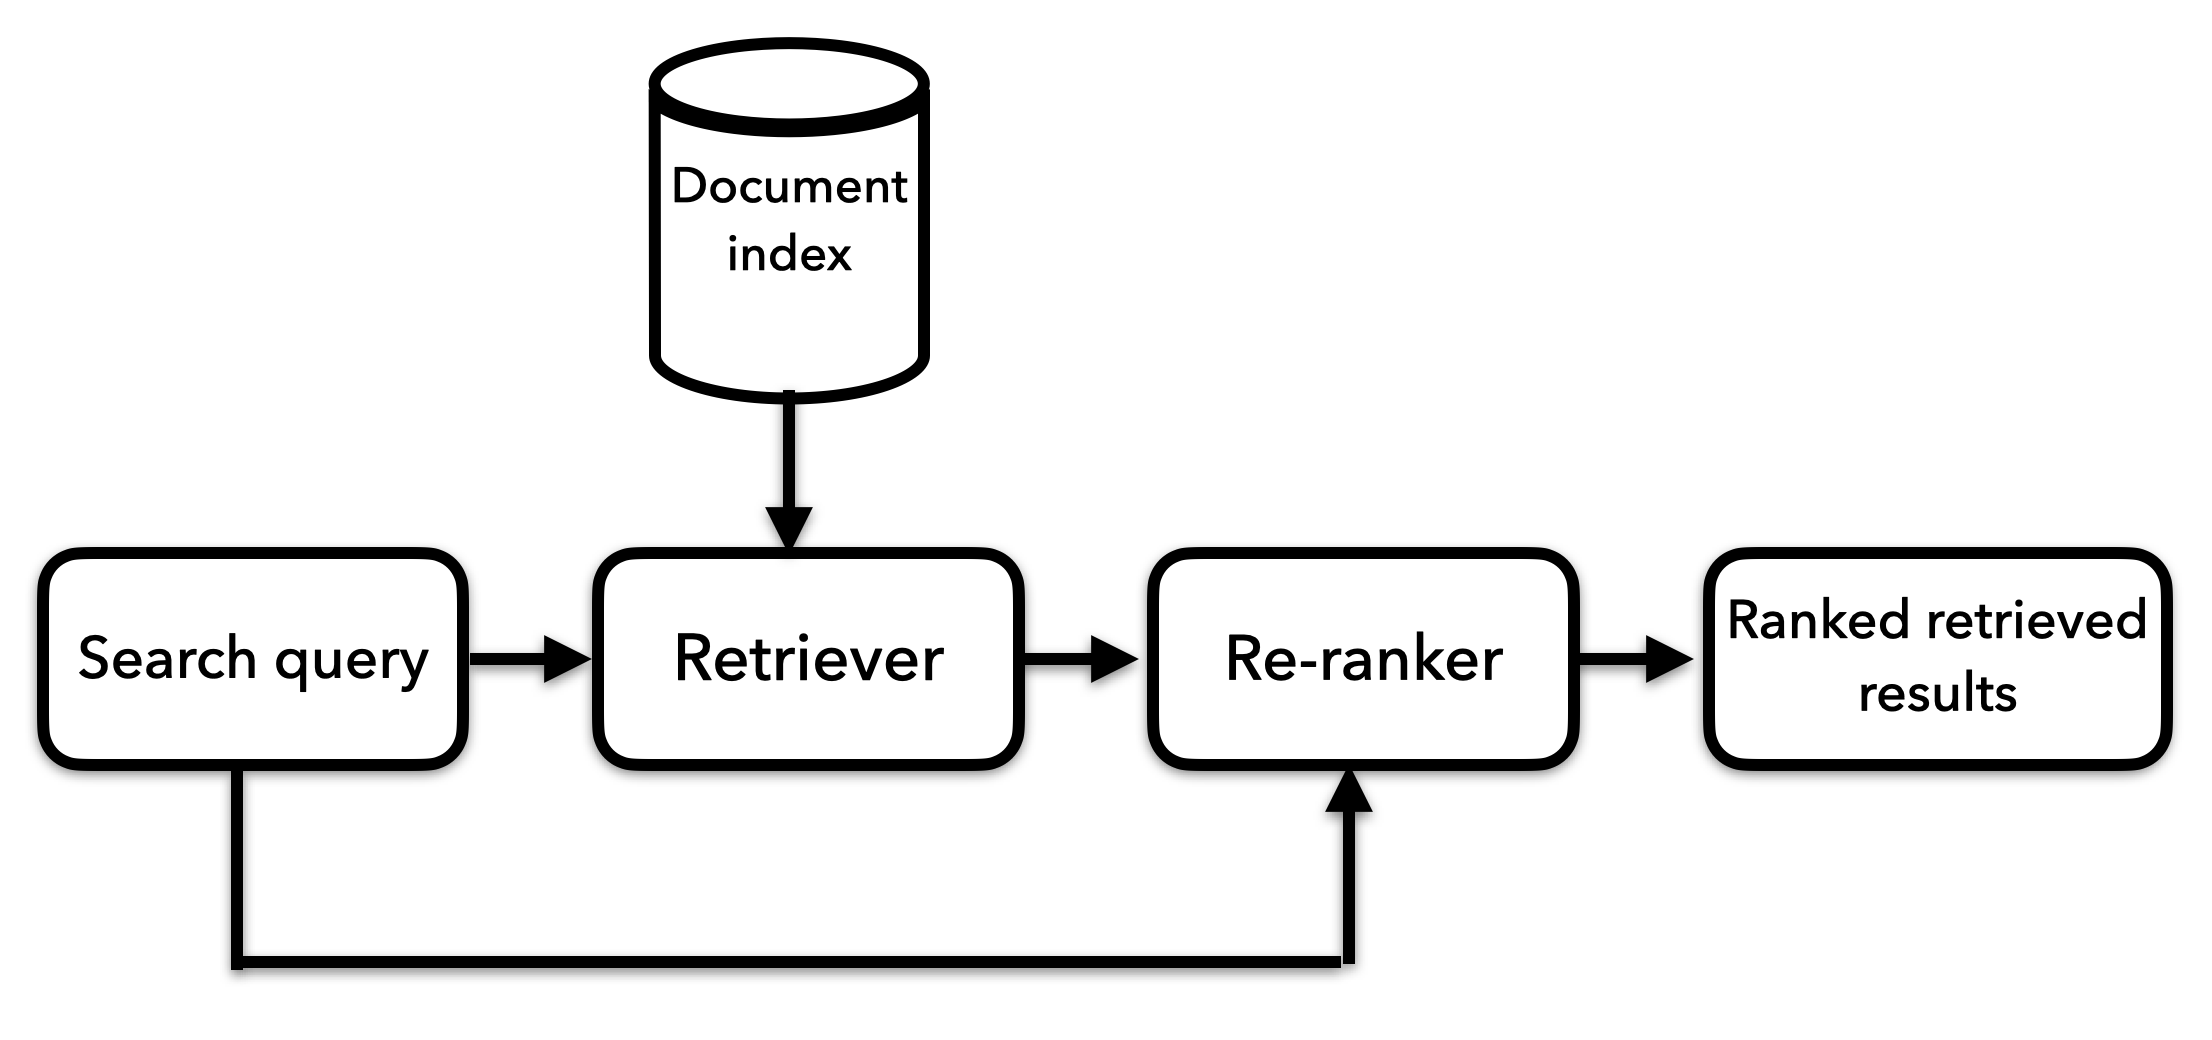
\includegraphics[width=.95\textwidth]{images/thesis_images/retriever_reranker_approach.png}
	\caption{Multi-stage ranking architecture.  \label{fig:multi-stage-ranking}}
\end{figure}

The retriever component is responsible for retrieving documents that are similar to the search query and generating a set of candidate texts for ranking~\cite{yates2021pretrained}. Various retrieval algorithms, such as BM-25 and bi-encoder semantic retrieval, can be employed at this stage. On the other hand, the re-ranker component organizes the candidate texts based on their relevance to the query~\cite{yates2021pretrained}. Re-ranker models often utilize transformer models that directly assign a relevance score to measure the alignment between the candidate text document and the query~\cite{nogueira2019passage, yates2021pretrained}. Unsupervised re-ranker models, known as cross-encoder, are pre-trained on retrieval datasets. This architecture has also been applied to enhance question-answering tasks. Malloci et al.~\cite{malloci2020text} utilized a specific candidate selection approach that filters phrases from keyword extraction by focusing on particular noun chunks. The pipeline employed in this research is illustrated in  \ref{fig:syntactic_candiate_selection}. 

\begin{figure}[h]
	\centering
	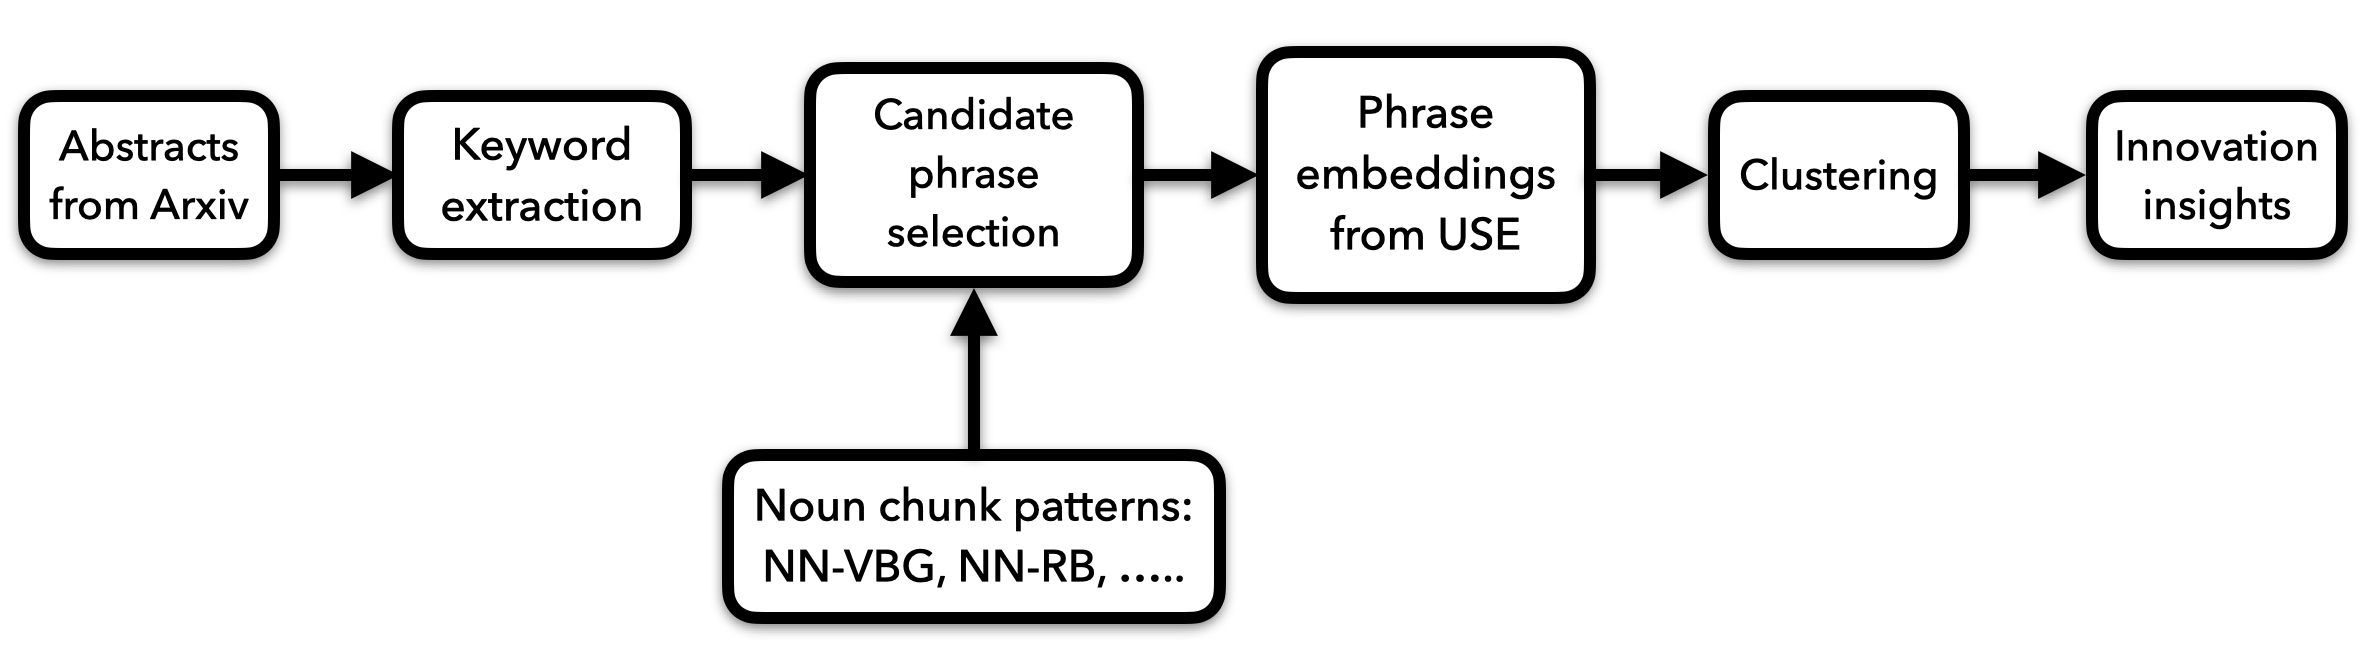
\includegraphics[width=.99\textwidth]{images/thesis_images/syntactic_candidate_selection.png}
	\caption[Innovation insights pipeline extraction.]{Pipeline to extract innovation insights using candidate selection.   \label{fig:syntactic_candiate_selection}}
\end{figure}

The primary purpose of this pipeline is to extract valuable insights related to innovation from research projects. The authors have provided detailed guidelines for selecting specific noun-chunk patterns to restrict the choice of keywords used in the clustering process. However, this approach has a limitation as it lacks semantic considerations during keyword selection, which may result in the exclusion of important keywords. Given the focus on innovation at \ac{FKIE}, this master thesis introduces and evaluates a unique query-specific candidate keyword selection approach. An important observation from the literature is the effectiveness of multi-stage ranking and the utilization of vector representations for text documents.

Furthermore, the proposed approach allows for the semantic mapping of documents to specific topics and accommodates multiple languages by utilizing a single multilingual pre-trained sentence encoder. This enables the seamless integration of news articles from various languages into the document indices, without requiring any modifications to the clustering pipeline. The proposed approach can be further expanded to analyze any corpus comprising long text documents associated with a given phrase or keyword. Given the lack of labeled news-articles with query and innovation relevance, an unsupervised approach is developed to establish an effective candidate document pool, facilitating efficient sub-topic creation and ranking. In subsequent sections, the proposed approach is described in detail and compared with existing literature.
